\chapter{Versuchsergebnisse}
\label{chap:testing}

Im Anschluss an die Implementierung der verschiedenen Algorithmen, sollten diese unter realen Bedingungen getestet werden. 
Dazu wurde ein Versuchsaufbau innerhalb eines Gebäudes aufgebaut, welches aus mehreren Räumen besteht. Dafür werden 9 Beacons innerhalb des Gebäudes verteilt. 
In der Offline-Phase werden dabei für jede Position 40 Fingerprints gesammelt, jeweils 10 in 90 Grad gedrehten Ausrichtungen.

Untersucht werden soll dabei zum einen die Genauigkeit der Positionierung eines sich bewegenden Objektes. Hierfür wird der Pfad aufgezeichnet und mit dem realen Pfad verglichen.
Zum Anderen soll die Positionierung an einer statischen Position getestet werden. Dazu wird an verschiedenen Testpunkten geprüft, ob die ausgegebene Position mit der realen Position übereinstimmt.

Der Testraum besteht dabei aus drei benachbarten Zimmern, wobei zwei dieser Zimmer durch ein offenen Durchgang verbunden sind. Das andere Zimmer ist über eine Tür zu erreichen. 
In Abbildung \ref{messraum} lässt sich der Aufbau des Messraumes erkennen, wobei die Dreiecke die eingemessenen Positionen darstellen und die Beacons als blaue Antennen gezeigt werden.

\begin{figure}[htb!]
		\centering
	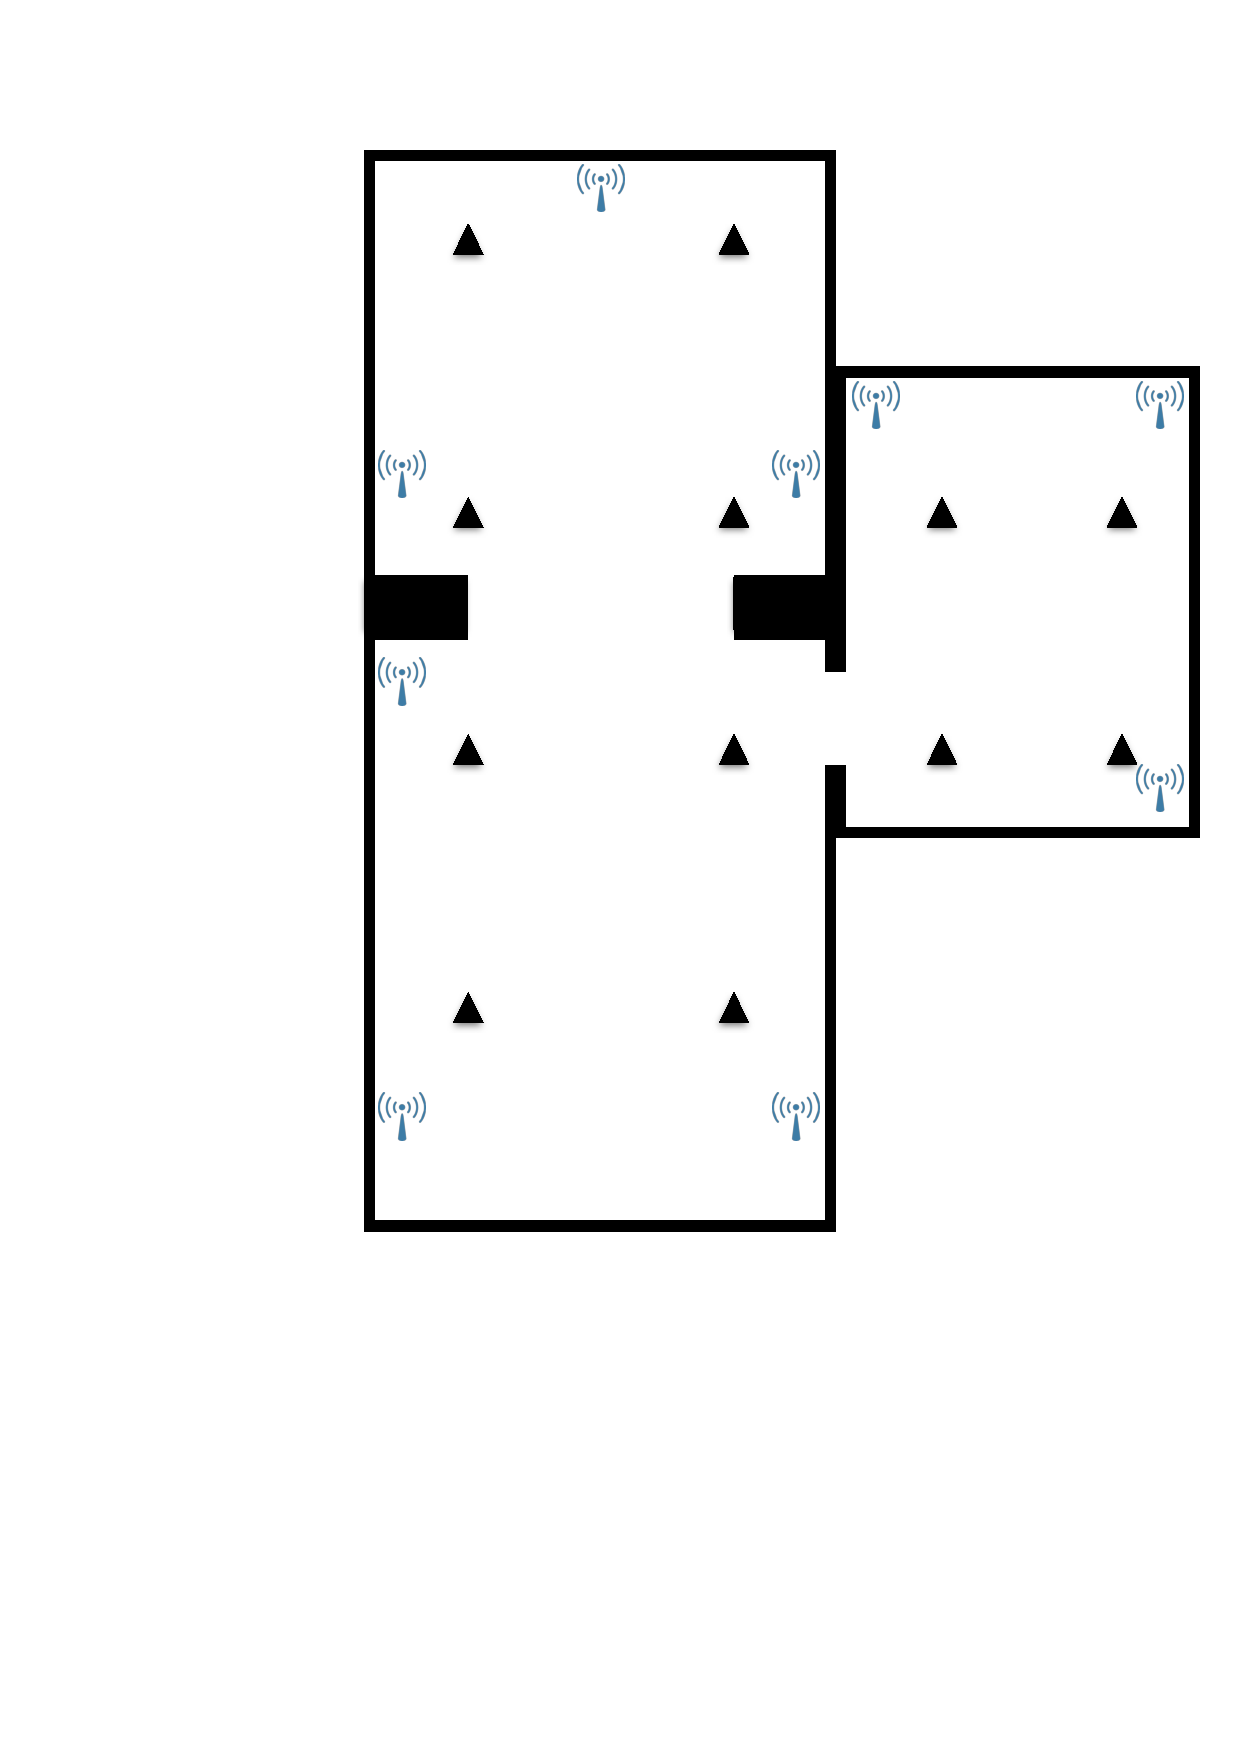
\includegraphics[scale=0.5]{messraum}
	\caption{Abbildung der Messraumes}
	\label{messraum}
\end{figure}

Die Abstände zwischen den einzelnen Messpositionen betragen dabei zwei Meter, woraus sich auch die mögliche Genauigkeit der Messung ergibt.

%%%%%%%%%%%%%%%%%%%%%%%%%%%%%%%%%%%%%%%%%%%%%%%%%%%%%%%%%%%%
\section{Positionierung eines beweglichen Objektes}
\label{sec:testing:moving}
%%%%%%%%%%%%%%%%%%%%%%%%%%%%%%%%%%%%%%%%%%%%%%%%%%%%%%%%%%%%

Bei den Tests der Positionierung bei einem bewegenden Objekt wird zuerst ein abzulaufender Pfad festgelegt, welcher jeweils über die Mittelpunkte der zuvor eingemessenen Zellen führt. Dieser Pfad wird dabei langsam abgelaufen und die Positionierungsangabe für jeden Algorithmus werden aufgezeichnet und nach Beendigung der Messungen wird der gemessene Pfad mit dem realen Pfad verglichen. Dabei wird das Hauptaugenmerk auf die Korrektheit der Position, die Größe der Abweichung und die Echtzeitfähigkeit des verwendeten Algorithmus gelegt.

Bei der Durchführung wurde zwei vorgegebene Wege abgelaufen. Bei der Analyse wird dabei der real abgeschrittene Weg mit dem, durch die Algorithmen errechneten, Weg verglichen.

Alle getesteten Algorithmen unterlagen dabei relativ starken Schwankungen zwischen einzelnen Zelle. Das Verfahren mittels Wahrscheinlichkeitsverteilungen erreichte bei diesem Test die höchste Genauigkeit, wobei hier die errechnete Position immer wieder zwischen der Zelle der aktuellen Position und den benachbarten Zellen wechselte. Durch diese Ungenauigkeit war es daher nicht möglich den genauen Laufweg zu reproduzieren. Eine Aussage darüber, in welchem Raum sich das Gerät aktuell befindet, konnte jedoch mit sehr großer Sicherheit durchgeführt werden.

Auch das Nearest-Neighbor-Verfahren über die gesamte Fingerprintdatenbank erlaubte ähnliche Aussagen zu treffen, obwohl es etwas instabiler als das probabilistische Verfahren ist. Der Vorteil dieses Systems ist die schnellere Aktualisierungsrate, da es nur auf den letzten gemessenen Wert zurückgreift. Das probabilistische Verfahren hingegen nutzt die letzten fünf gemessenen Werte, wodurch sich die Aktualisierung der Position um einige Sekunden verzögert.

Das Nearest-Neighbor-Verfahren über die Mittelwert schnitt bei dieser Untersuchung schlecht ab. Eine Positionsangabe war kaum möglich, da die Zellenangaben stark schwankten und im Großteil der Fälle ein falsche Position anzeigt wurde.


Bei der Positionierung von beweglichen Objekten ist der probabilistische Algorithmus am Besten geeignet, da dieser einen guten Kompromiss zwischen Genauigkeit und Aktualisierungsrate bietet. Falls mehr Wert auf eine sehr schnell Aktualisierung gelegt wird, sollte jedoch der Nearest-Neighbor-Algorithmus über alle Fingerprints genutzt werden, da dieser eine sofortige Aktualiserung der Position mit sich bringt.

%%%%%%%%%%%%%%%%%%%%%%%%%%%%%%%%%%%%%%%%%%%%%%%%%%%%%%%%%%%%
\section{Statische Positionierung}
\label{sec:testing:static}
%%%%%%%%%%%%%%%%%%%%%%%%%%%%%%%%%%%%%%%%%%%%%%%%%%%%%%%%%%%%

Bei der statischen Positionierung wird an verschiedenen festen Positionen eine Positionsmessung durchgeführt. Dabei werden die Ergebnisse der verschiedenen Algorithmen verglichen. Es wird neben der korrekten Positionsangabe besonders auf die Konstanz dieser Positionsangabe geachtet. Diese sollte nicht zu stark schwanken und sich nach kurzer Zeit auf die korrekte Position einpendeln.

Bei der Untersuchung der statischen Positionierung wurde an vier verschiedenen Punkten im Messraum für 20 Sekunden Stichproben genommen. Dabei wurden alle implementierten Algorithmen untersucht und direkt verglichen.

Es wird eine grobe Unterteilung genutzt, sodass eine Positionierung entweder die richtige Zelle bestimmt, eine benachbarte Zelle oder eine weiter entfernte Zelle als aktuelle Position angibt. 

Wie bereits erwartet, schnitt der Algorithmus mit der Wahrscheinlichkeitsverteilung am Besten ab. Dieser schaffte es in knapp zwei Drittel der Fälle die genaue Position zu bestimmen. In den restlichen Fällen bestimmte der Algorithmus eine benachbarte Position als aktuelle Position. Dabei wurde kein Mal eine nicht in unmittelbarer Nachbarschaft befindliche Position als aktuelle Zelle angenommen. 

Überraschender Weise liegt der Nearest-Neighbor-Algorithmus, welcher über alle Fingerprints iteriert, von der Genauigkeit an der zweiten Stelle. Die Quote der richtigen Positionsangaben lag dabei bei etwa 50 Prozent. In etwa 40 Prozent der Fälle wurde eine benachbarte Position als die aktuelle Position bestimmt und nur in einem Zehntel der Fälle wurde eine Position, welche sich nicht in der direkten Nachbarschaft befindet, bestimmt.
Der Nearest-Neighbor-Algorithmus mit dem Median und der durchschnittlichen Signalstärke lagen bei der Messung gleich auf. Dabei ergab sich bei dieser Methode nur eine Treffrate von 36 Prozent. Als benachbarte Zelle werden nur etwa 5 Prozent der erkannten Positionen bestimmt. Die Fehlerquote dieser Methode liegt dabei bei über der Hälfte aller bestimmten Positionen und ist so nicht ausreichend genau.

% \begin{tabular}{lcr}
%   & Nearest-Neighbor für alle Fingerprint & Nearest-Neighbor für Median und Durchschnittswerte & Wahrscheinlichkeitsmethode \\
%   Genaue Zelle & 51,3 & 36,8 & 68,4 \\
%   Benachbarte Zelle & 39,5 & 52,6 & 31,6 \\
%   Entfernte Zelle & 9,2 & 57,9 & 0 \\
% \end{tabular}
\begin{figure}[htb!]
		\centering
	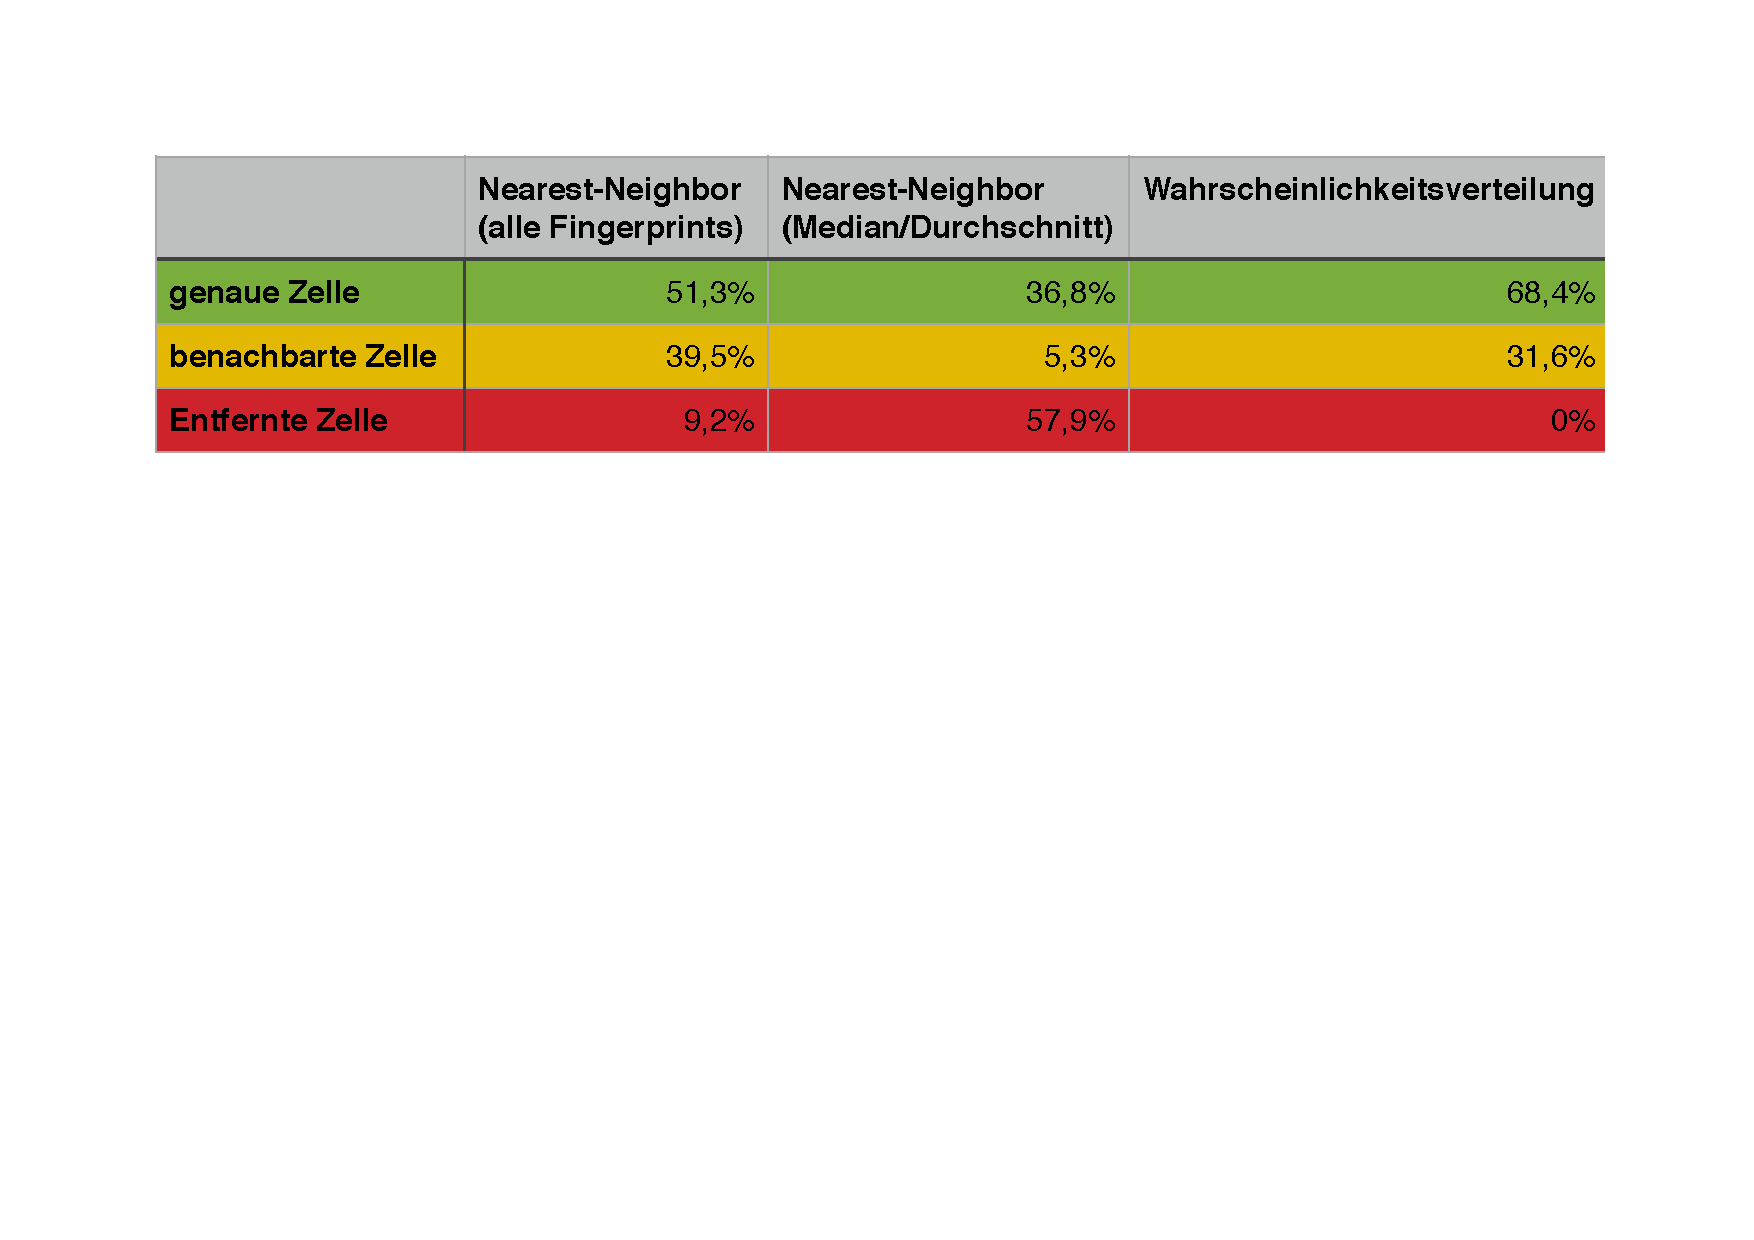
\includegraphics[scale=0.5]{statistic-static}
	\caption{Genauigkeitswerte der statischen Lokalisierung}
	\label{statistic-static}
	\end{figure}
 
Für eine statische Positionierung ist das Verfahren zur Positionierung mittels Wahrscheinlichkeitsverteilungen sehr gut geeignet. Die Genauigkeit ist dabei ausreichend, da der größte gemessene Fehler eine Lokalisierung in eine benachbarten Zelle ist. Außerdem ist dieses Verfahren relativ robust und es sind nur geringe Schwankungen in der Positionierung zu beobachten.

Auch das Nearest-Neighbor-Verfahren über die gesammte Datenbank der Fingerprints liefert akzeptable Ergebnisse und liegt nur in unter 10 Prozent der Fälle außerhalb der eigentlichen oder benachbarten Zelle. Hierbei sind jedoch schon größere Schwankungen zu erkennen, sodass die Positionierung häufiger zwischen zwei oder mehreren Zelle springt.

Die Nearest-Neighbor-Methode mit den Mittelwerte ist weniger geeignet für die Indoor Positionierung, da hier eine sehr hohe Fehlerrate vorliegt und die Ergebnisse zudem sehr stark schwanken.